\documentclass[usenames,dvipsnames]{beamer}

\mode<presentation>
{
\usetheme[width=0.7in]{Hannover}
  \setbeamercovered{transparent}
}
\usepackage{longtable}
\usepackage{booktabs}
% \usepackage{bnf}
\usepackage{bm}

\usepackage[english]{babel}
\usepackage[latin1]{inputenc}

\usepackage{times}

\usepackage{multirow}
\usepackage{totpages}
\usepackage{hyperref}
\usepackage{booktabs}
\usepackage[round]{natbib}

%\usepackage{listings}
%\lstset{frame=none, showstringspaces=false, basicstyle=\ttfamily\bfseries\footnotesize,
%  xleftmargin=-8mm,language=Haskell,breaklines=true}

\usepackage{tikz}
\usetikzlibrary{positioning}

\hypersetup{colorlinks=true,
    linkcolor=blue,
    citecolor=blue,
    filecolor=blue,
    urlcolor=blue,
    unicode=false}

% \usepackage{pifont}
\usepackage{amsmath, amsfonts, amssymb, xspace, xcolor, url}
\newcommand{\cross}{{\LARGE {\color{red}\ding{55}}}}

\newcommand{\greencheck}{{\LARGE {\color{ForestGreen}\checkmark}}}
\newcommand{\bluedash}{{\LARGE {\color{blue}{--}}}}

\newcommand{\blt}{- } %used for bullets in a list

\newcommand{\colAwidth}{0.1\textwidth}
\newcommand{\colBwidth}{0.8\textwidth}

\renewcommand{\arraystretch}{1.1} %so that tables with equations do not look crowded

\title{Generating Software for Well-Understood Domains}

%\subtitle
%{Include Only If Paper Has a Subtitle}

\author{\textbf{Jacques Carette}, W. Spencer Smith, Jason Balaci}

\institute[McMaster University]
{
  Computing and Software Department\\
  McMaster University
}
% - Keep it simple, no one is interested in your street address.

\date[EVCS 2023] % (optional, should be abbreviation of conference name)
{EVCS 2023}

\subject{research software, software engineering, code generation, domain engineering}
% This is only inserted into the PDF information catalog. Can be left
% out. 

% If you have a file called "university-logo-filename.xxx", where xxx
% is a graphic format that can be processed by latex or pdflatex,
% resp., then you can add a logo as follows:

%\pgfdeclareimage[height=0.5cm]{Mac-logo}{McMasterLogo}
%\logo{\pgfuseimage{Mac-logo}}

% Delete this, if you do not want the table of contents to pop up at
% the beginning of each subsection:
% \AtBeginSubsection[]
% {
%   \begin{frame}<beamer>
%     \frametitle{Outline}
%     \tableofcontents[currentsection,currentsubsection]
%   \end{frame}
% }

% If you wish to uncover everything in a step-wise fashion, uncomment
% the following command: 

%\beamerdefaultoverlayspecification{<+->}

\beamertemplatenavigationsymbolsempty 

\begin{document}

%%%%%%%%%%%%%%%%%%%%%%%%%%%%%%%%%%%%%%
\hoffset=-.4in %removing side bar for these frames
\begin{frame}[plain]

%\begin{tikzpicture}[remember picture,overlay]
%  \node [xshift=1.3cm,yshift=0cm] at (current page.center)
%  {
%  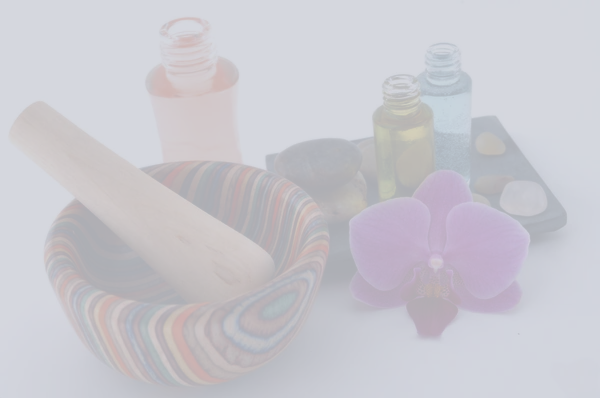
\includegraphics[width=1.5\textwidth]{holisticFaint.png}
%  };
%\end{tikzpicture}

\titlepage

\end{frame}
\hoffset=0in %restore
%%%%%%%%%%%%%%%%%%%%%%%%%%%%%%%%%%%%%%

%\hoffset=-.4in %removing side bar for these frames
%\begin{frame}[plain]
%  
%  \frametitle{Example}
%  
%  \hspace{-1.1cm}
%  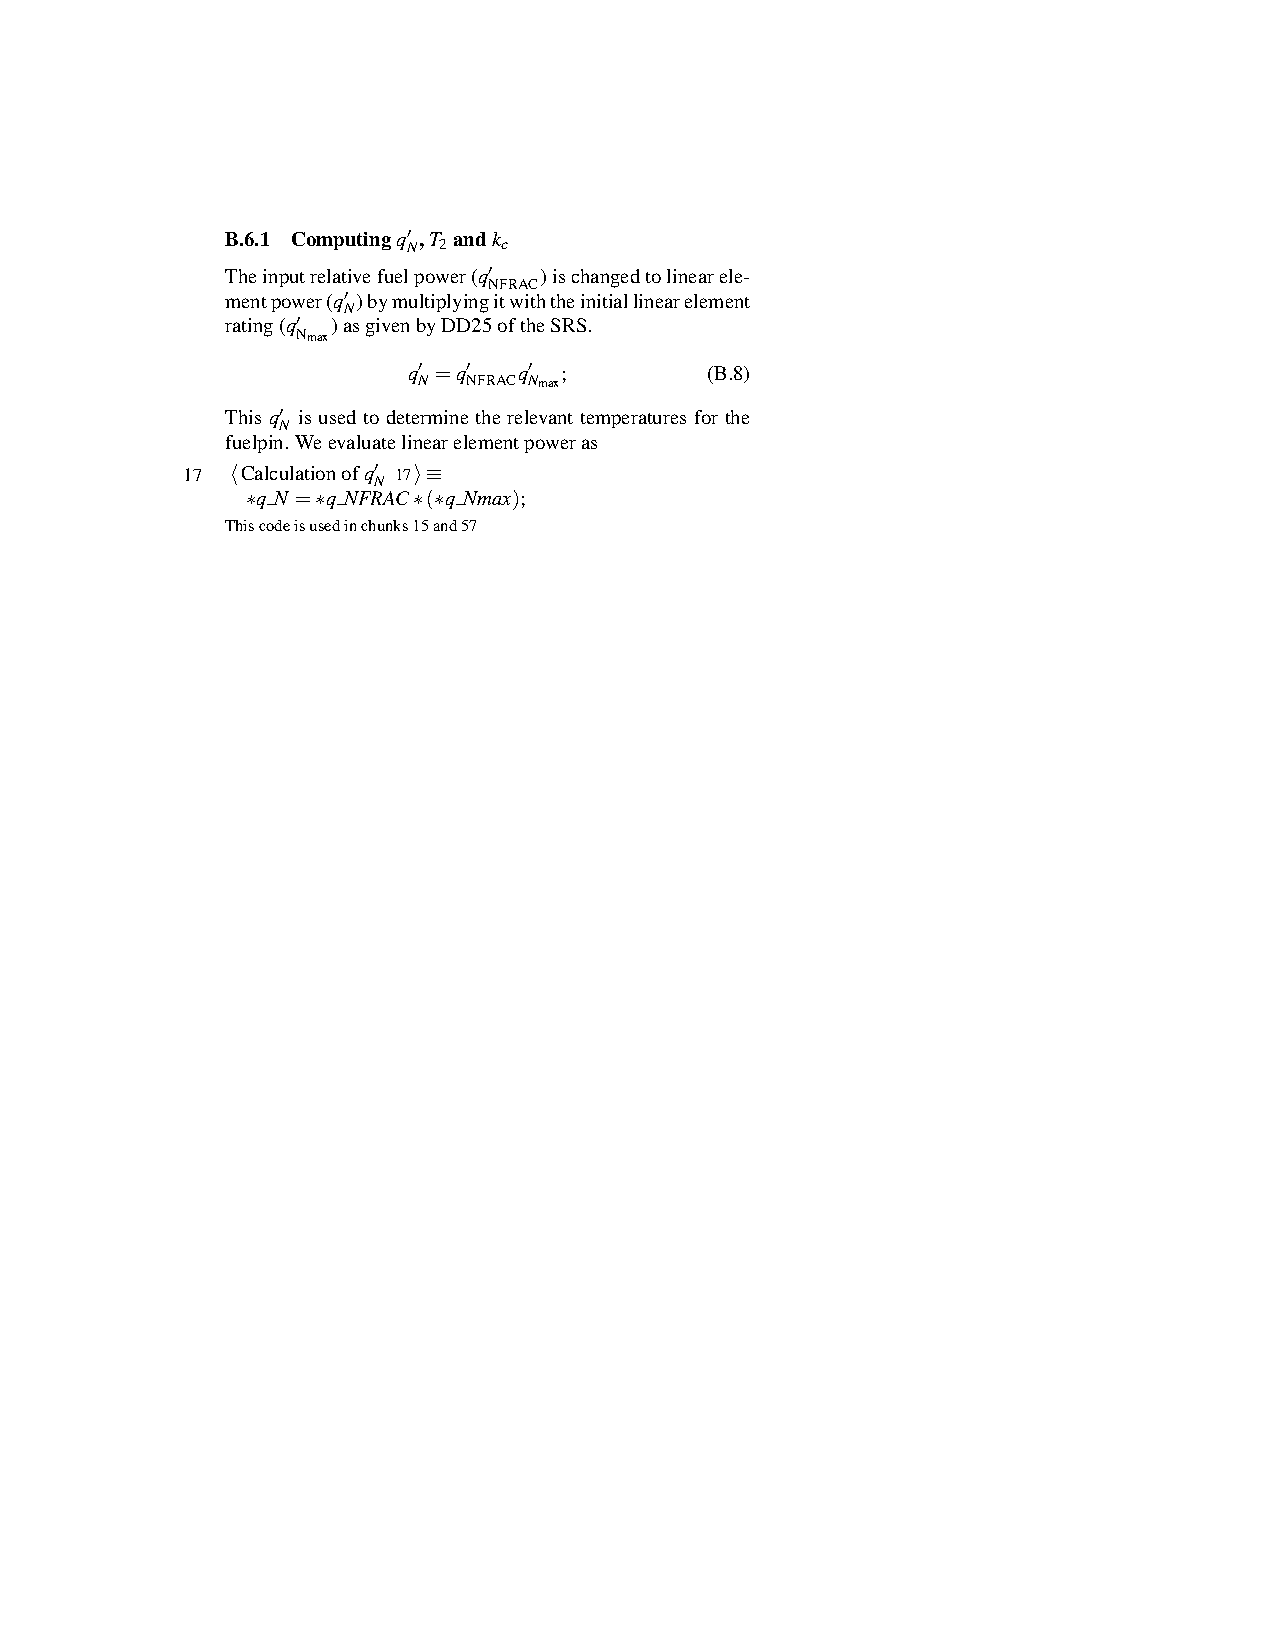
\includegraphics[width=1.1\columnwidth]{qnfrac.pdf}
%  
%\end{frame}
%\hoffset=0in %restore

%%%%%%%%%%%%%%%%%%%%%%%%%%%%%%%%%%%%%%%%%%%%%%%%%%%%%%%%%%%%%%
  
\begin{frame}
  
  \frametitle{Calculations}
  
  Given $F, Q, \kappa, \phi, \gamma$ calculate:

  \begin{equation} \label{EqImplicitFEM}
    \mathbf{K} = \int_V \mathbf{B}^T \mathbf{D}^{vp} \mathbf{B} dV; \mathbf{F} = \mathbf{R}_i - \int_V \mathbf{B}^T \bm{\sigma}_i dV + \int_V \mathbf{B}^T
    \Delta
    \bm{\sigma}^{vp} dV
    \end{equation}
    with
    \begin{equation}
    \mathbf{D}_{vp} =
    \mathbf{D} \left [
    \mathbf{I} - {\Delta t} C_1 \lambda' \frac{\partial Q}{\partial \bm{\sigma}} \left ( \frac{\partial F}{\partial
    \bm{\sigma}} \right )^{T} \mathbf{D}
    \right ], \lambda' = \frac{d \lambda}{d F}
    \end{equation}
    \begin{equation}
    \Delta \bm{\sigma}^{vp} = \Delta t C_1 \lambda \mathbf{D} \frac{\partial Q}{\partial \bm{\sigma}}
    \end{equation}
    \begin{equation}
    C_1 = [1 + \lambda' {\Delta t} (H_e + H_p)]^{-1}
    \end{equation}
    \begin{equation}
    \label{HEE}
    H_e = \left ( \frac{\partial F}{\partial \bm{\sigma}} \right )^T \mathbf{D} (\frac{\partial Q}{\partial \bm{\sigma}})
    \end{equation}
    \begin{equation}
    H_p = -\frac{\partial F}{\partial \kappa} \left ( \frac{\partial \kappa}{\partial \bm{\epsilon}^{vp}}
    \right )^T \frac{\partial Q}{\partial \bm{\sigma}}
    \end{equation}
    %where $\mathbf{I}$ is the identity matrix.
  
  \end{frame}
  
  
%%%%%%%%%%%%%%%%%%%%%%%%%%%%%%%%%%%%%%

\begin{frame}

\frametitle{Holistic Approach}

\hspace{-1cm}
\begin{itemize}
\item Combine 
\begin{itemize}
  \item Lit programming emphasis on documentation
  \item Code gen, but for everything
\end{itemize}
\item Codify more knowledge
\begin{itemize}
\item Physics knowledge
\item Computing knowledge
\item Document knowledge %(more than org mode)
\item Design knowledge
\item Traceability knowledge
\item Technology knowledge %(makefiles, testing frameworks, CI, etc.)
\end{itemize}

\end{itemize}

\begin{tikzpicture}[remember picture,overlay]
  \node [xshift=3.4cm,yshift=-2.0cm] at (current page.center)
  {
  
\includegraphics[width=0.47\textwidth]{generate_all_the_things.jpg}
  };
\end{tikzpicture}

\end{frame}

%%%%%%%%%%%%%%%%%%%%%%%%%%%%%%%%%%%%%%
\hoffset=-.4in %removing side bar for these frames    
\begin{frame}[plain] % knowledge duplication

  \begin{tikzpicture}[remember picture,overlay]
    \node [xshift=0.8cm,yshift=0.0cm] at (current page.center)
    {
    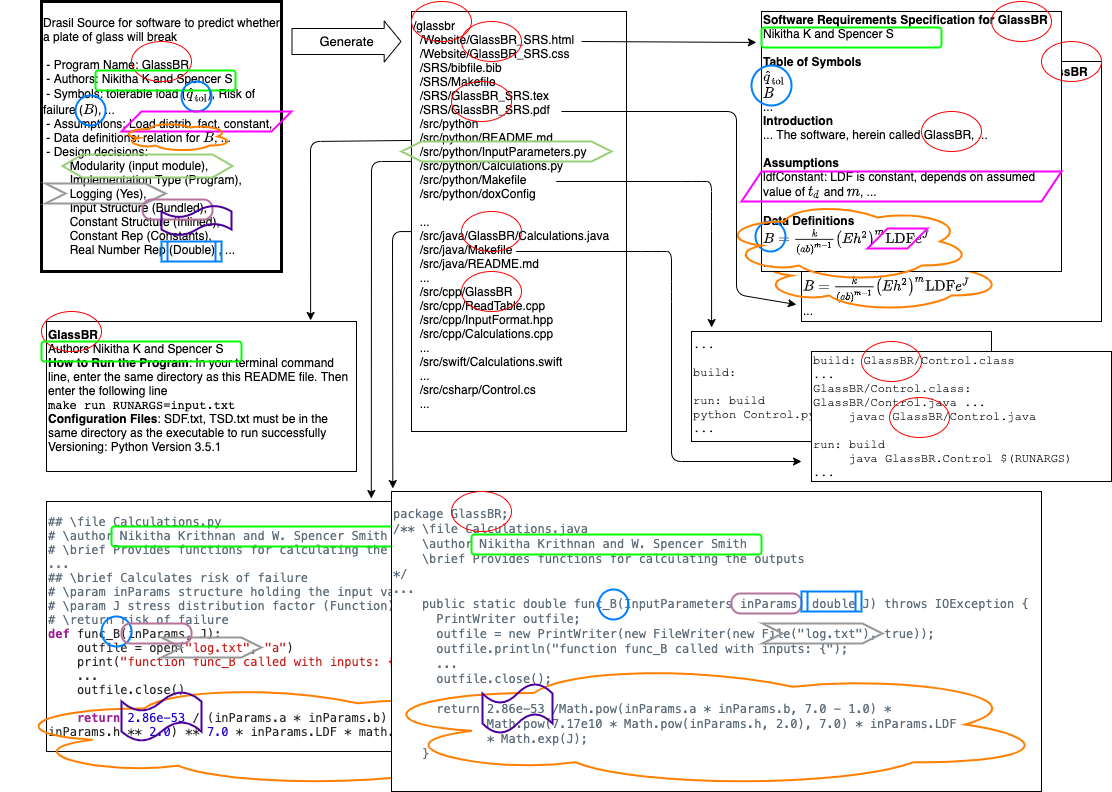
\includegraphics[width=1.2\textwidth]{DrasilSupportsChange.png}
    };
  \end{tikzpicture}
  
\end{frame}
\hoffset=0in %restore  

\end{document}
